\chapter{Beam Lines, Sequences, and Ranges}
\label{sec:lines}
\index{line|(}

\section{Beam Lines}
\label{sec:line}
\index{LINE}

The accelerator to be studied is known to \opal
as a sequence of physical elements called a \textbf{beam line}.
A beam line is built from simpler beam lines whose definitions
can be nested to any level.
A powerful syntax allows to repeat or to reflect pieces of beam lines.
Formally a beam line is defined by a \texttt{LINE} command:
\begin{verbatim}
label:LINE=(member,...,member);
\end{verbatim}
\secref{\texttt{label}}{label} gives a name to the beam line 
for later reference.

Each \texttt{member} may be one of the following:
\begin{itemize}
\item An element label,
\item A beam line label,
\item A \secref{\texttt{SEQUENCE}}{sequence} label,
\item A sub-line, enclosed in parentheses,
\end{itemize}
Beam lines can be nested to any level.

\subsection{Simple Beam Lines}
\label{sec:simple}
The simplest beam line consists of single elements:
\begin{verbatim}
label:LINE=(member,...,member);
\end{verbatim}
Example:
\begin{verbatim}
L:LINE=(A,B,C,D,A,D);
TWISS,LINE=L;
\end{verbatim}
The \secref{\texttt{TWISS} command}{twiss} tells \opal to perform
lattice calculations on the sequence 
\begin{verbatim}
A,B,C,D,A,D
\end{verbatim}

\subsection{Sub-lines}
\label{sec:subline}
Instead of referring to an element,
a beam line member can refer to another beam line
defined in a separate command.
This provides a shorthand notation for sub-lines which occur
several times in a beam line.
Lines and sub-lines can be entered in any order,
but when a line is used,
all its sub-lines must be known.

Example:
\begin{verbatim}
L:LINE=(A,B,S,B,A,S,A,B);
S:LINE=(C,D,E);
TWISS,LINE=printL;
\end{verbatim}
This example produces the following expansion steps:
\begin{enumerate}
\item Replace sub-line \texttt{S}:
\begin{verbatim}
(A,B,(C,D,E),B,A,(C,D,E),A,B)
\end{verbatim}
\item Omit parentheses:
\begin{verbatim}
A,B,C,D,E,B,A,C,D,E,A,B
\end{verbatim}
\end{enumerate}

\subsection{Reflection and Repetition}
\label{sec:refrep}
An unsigned repetition count and an asterisk indicate
repetition of a beam line member.
An optional minus sign (\texttt{-}) prefix causes reflection,
i.e. all elements in the subsequence are taken in reverse order.
Sub-lines of reflected lines are also reflected,
but on physical elements the reflection flag is ignored.
The minus sign must precede any repetition count.
Repetitions are expanded immediately when a line is read,
so are reflections of anonymous beam lines.
The result is a flat line referring to a sequence of named elements and/or
beam lines.
Please note this is not yet supported for \noopalt and \noopalcycl .
When the line is output, it has the form resulting from this expansion.

Example:
\begin{verbatim}
R:LINE=(G,H);
S:LINE=(C,R,D);
T:LINE=(2*S,2*(E,F),-S,-(A,B));
TWISS,LINE=T;
\end{verbatim}
The three lines are stored as follows:
\begin{verbatim}
R:LINE=(G,H);
S:LINE=(C,R,D);
T:LINE=(S,S,E,F,E,F,-S,B,A);
\end{verbatim}
When \texttt{T} is expanded, substitution is recursive:
\begin{enumerate}
\item Replace sub-line \texttt{S}:
\begin{verbatim}
(C,R,D,C,R,D,E,F,E,F,D,-R,C,B,A)
\end{verbatim}
\item Replace sub-line \texttt{R}:
\begin{verbatim}
(C,G,H,D,C,G,H,D,E,F,E,F,D,H,G,C,B,A)
\end{verbatim}
\end{enumerate}
Note that the inner sub-line R is reflected together with
the outer sub-line S.
\index{line|)}

\section{Beam Line Sequences}
\label{sec:sequence}
\index{SEQUENCE}
\index{sequence|(}
A sequence of elements can easily be generated from a data base
using a command looking like
\begin{verbatim}
label:SEQUENCE,REFER=keyword,L=expression,REFPOS=name;
   object-definition;
   ...;
   object-definition;
ENDSEQUENCE;
\end{verbatim}
It reads a sequence of element definitions,
compiles an object which resembles a beam line definition,
and gives it the name "label".
The resulting sequence can be used like a beam line.
Please note this is not yet supported for \noopalt and \noopalcycl .
The attributes of the sequence are:
\begin{description}
\item[REFER]
  \index{REFER}
  The reference points for the elements are specified by the \texttt{REFER} 
  attribute:
  \begin{description}
  \item[REFER=CENTRE]
    \index{CENTRE}
    The reference points are at the element centres (default).
  \item[REFER=ENTRY]
    \index{ENTRY}
    The reference points are at element entrances.
  \item[REFER=EXIT]
    \index{EXIT}
    The reference points are at element exits.
  \end{description}
\item[L]
  \index{L}
  The length of the \texttt{SEQUENCE} can be given on the 
  \texttt{SEQUENCE} command,
  or it may be entered with the \texttt{ENDSEQUENCE} command.
\item[REFPOS]
  \index{REFPOS}
  Normally, the reference position for a nested sequence is defined by
  the \texttt{REFER} attribute of the enclosing sequence,
  but, if \texttt{REFPOS} is given, it specifies a \textbf{unique}
  element in the sequence whose \texttt{AT} attribute becomes the 
  reference point for the sequence.
\end{description}
For each non-drift element in the sequence one element definition appears
following the \texttt{SEQUENCE} command and preceding the
\texttt{ENDSEQUENCE} command. 
These look similar to ordinary \secref{element definitions}{element},
but they may contain an optional specification to place the element:
\begin{verbatim}
class-name,AT=expression;
class-name,AT=expression,FROM=name;
class-name,DRIFT=expression;

object-name,class-name,
	AT=expression,attribute,...,attribute;
object-name,class-name,
	AT=expression,FROM=name,attribute,...,attribute;
object-name,class-name,
	DRIFT=expression,attribute,...,attribute;
\end{verbatim}
The meaning of the \texttt{AT} specifications is:
\begin{description}
\item[AT=expression]
  \index{AT}
  Place the element's entrance, centre, or exit at the specifiet
  position.
\item[FROM=name]
  \index{FROM}
  Interpret the \texttt{AT} specification as relative to the
  \textbf{unique} element \texttt{name}.
\item[FROM=\#S]
  \index{\#S}
  Like omitting the \texttt{FROM} specification, \texttt{AT} is
  relative to the beginning of the sequence.
\item[FROM=\#E]
  \index{\#E}
  The \texttt{AT} specification is relative to the end of the
  sequence. 
\item[FROM=PREVIOUS]
  \index{PREVIOUS}
  The \texttt{AT} specification is relative to the previous element.
\item[FROM=NEXT]
  \index{NEXT}
  The \texttt{AT} specification is relative to the following element.
\item[DRIFT=expression]
  \index{DRIFT}
  The element is preceded by a drift of the given length.
\end{description}

One should consider the following:

\begin{enumerate}
\item The name \texttt{class-name} must be an element 
  \secref{class name}{elm-class}, 
  it may optionally be preceded by a minus sign (\texttt{-}).
  This  inverts the order of the elements in the inserted object.
  This makes sense only for a beam line or sequence.
  
\item If the name \texttt{object-name} is not given,
  \opal inserts the element specified by \texttt{class-name}.
  In this case no further attributes are allowed.
  
\item If there is a non-blank \texttt{object-name},
  this name should not be defined earlier in the data.
  \opal then first makes a copy of \texttt{class-name} and gives it 
  the new name \texttt{object-name}.
  Any further attributes override the attributes inherited from 
  \texttt{class-name}.b
  
\item The elements must be entered in order of increasing position,
  and they must not overlap.
  Their positions are evaluated while reading the \texttt{SEQUENCE}
  definition, and become \textbf{constant} values.
  
\item A \secref{\texttt{LINE}}{line} or
  \secref{\texttt{SEQUENCE}}{sequence} can be nested in another
  \texttt{SEQUENCE} or \texttt{LINE}. 
\end{enumerate}

Within the \texttt{SEQUENCE}, 
\opal generates the drift spaces for proper positioning.

Example:
\begin{verbatim}
// Define element classes for a simple cell:
B:  SBEND,L=35.09,ANGLE = 0.011306116;
QF: QUADRUPOLE,L=1.6,K1=-0.02268553;
QD: QUADRUPOLE,L=1.6,K1=0.022683642;
SF: SEXTUPOLE,L=0.4,K2=-0.13129;
SD: SEXTUPOLE,L=0.76,K2=0.26328;
// Define the cell as a sequence:
CELL:SEQUENCE,L=79.0;
   B1: B, AT=19.115;
   SF1:SF,AT=37.42;
   QF1:QF,AT=38.70;
   B2: B, AT=58.255,ANGLE=-B1->ANGLE;
   SD1:SD,AT=76.74;
   QD1:QD,AT=78.20;
ENDSEQUENCE;
\end{verbatim}
In this example all members of the sequence have a new name,
and \opal generates copies of the corresponding classes.
The bending magnet \texttt{B1} is wrapped to change sign,
but its definition is still equal to \texttt{B}.
Thus \texttt{B2}, which has the negative field of \texttt{B1},
has the same effect as the wrapped element \texttt{B1}.
\index{sequence|)}

\section{Lines and Sequences with arguments}
\index{line!argument}
\index{sequence!argument}
\index{argument!line}
\index{argument!sequence}
A line or sequence definition can also have parameters like a
\secref{\texttt{MACRO}}{macro}.
Such a line or sequence can be nested (and instantiated) in another
line or sequence, but it \textbf{must have a unique name} when
instantiated in a sequence. 
\par
Examples:
\begin{verbatim}
CELL(X,Y):SEQUENCE,L=79;
   QF&X: QF,AT=...;            
   Y&X:  Y,L=1,AT=...;
   QD&X: QD,AT=...;
ENDSEQUENCE;
\end{verbatim}
When used as
\begin{verbatim}
CELL12: CELL(12,SF);
\end{verbatim}
this expands to
\begin{verbatim}
CELL12:SEQUENCE,L=79;
   QF12: QF,AT=...;            
   SF12: SF,L=1,AT=...;
   QD12: QD,AT=...;
ENDSEQUENCE;
\end{verbatim}
A second example:
\begin{verbatim}
CELL(X,Y):LINE=(D1,QF&X,D2,Y&X,D3,QD&X,D4);
\end{verbatim}
If the proper drifts are used, this example is equivalent to
the sequence example above.

\section{Shared Lines}
\label{sec:seq-class}
\index{line!shared}
\index{share lines}
\index{sequence!shared}
\index{shared sequences}
Please note this is not yet supported for \noopalt and \noopalcycl .
Normally, when a beam line or sequence is referred to in another line,
each reference refers to a \textbf{distinct} copy of the line.
\begin{verbatim}
L:LINE=(A,B,C);
S:SEQUENCE,L=real;
   ...
ENDSEQUENCE;
\end{verbatim}
Such a line or sequence is cloned when it is inserted in another line
or sequence, thus permitting assignment of errors to its elements
without affecting other occurrences of the same line.

A beam line or sequence can be shared by using the keyword
\texttt{SHARED},
\index{SHARED}
then the line or sequence is unique,
and all references in other lines refer to the \textbf{same} instance.
Example:
\begin{verbatim}
// Define the interaction region common to both rings:
SHARED IR2:SEQUENCE,L=...;
   ...
ENDSEQUENCE;
RING1:LINE=(...,IR2,...);
RING2:LINE=(...,IR2,...);
// Now assign imperfections to IR2 wich 
// will be seen by both rings:
EALIGN,LINE=IR2,DX=...,DY=...;
\end{verbatim}
Counterexample:
\begin{verbatim}
// Define one superperiod of the machine:
SUPER:SEQUENCE,L=...;
   ...
ENDSEQUENCE;
// Each occurrence of SUPER is distinct:
RING:LINE=(8*SUPER);
// Assign different imperfections to each SUPER:
EALIGN,LINE=RING,DX=...,DY=...;
\end{verbatim}

\section{Sequence Editor}
\label{sec:editor}
\index{edit!sequence}
\index{sequence editor|(}
\index{SEQEDIT}
\index{ENDEDIT}
Please note this is not yet supported for \noopalt and \noopalcycl .
During editing of a sequence, all element positions are evaluated 
immediately when defined and stored as \textbf{constant} values.
To modify a sequence it must be selected for editing by the command
\begin{verbatim}
SEQEDIT,SEQUENCE=old-name;
\end{verbatim}
\opal enters editing mode during which it only recognises the 
\tabref{sequence editor commands}{edit},
and makes the sequence \texttt{old-name} the current sequence being edited.
Editing mode is switched off by the command
\begin{verbatim}
ENDEDIT,NAME=new-name;
\end{verbatim}
If \texttt{new-name} is non-blank, it becomes the name of the edited sequence,
otherwise the modified sequence is stored under its old name.

\begin{table}[ht]
  \begin{center}
    \begin{tabular}{|p{0.3\textwidth}|p{0.6\textwidth}|}
      \hline
      Command & Purpose \\
      \hline
      \tabline{SELECT}{Select elements to be affected}{editselect}
      \tabline{CYCLE}{Change starting point (cyclic interchange)}{editcycle}
      \tabline{FLATTEN}{Flatten the sequence}{editflat}
      \tabline{INSTALL}{Install new elements}{editinstall}
      \tabline{MOVE}{Move elements}{editmove}
      \tabline{REFLECT}{Reflect the sequence}{editreflect}
      \tabline{REMOVE}{Remove elements}{editremove}
      \tabline{REPLACE}{Replace elements}{editreplace}
      \tabline{ENDEDIT}{Leave sequence edit mode}{editor}
      \hline
    \end{tabular}
    \caption{Commands accepted in editor mode}
    \label{tab:edit}
  \end{center}
\end{table}

\subsection{Selecting Element(s)}
\label{sec:editselect}
\index{SELECT}
Elements are selected by a command
\begin{verbatim}
SELECT,RANGE=range,CLASS=name,PATTERN=regex,
                FULL=logical,CLEAR=logical;
\end{verbatim}
When the clause \texttt{SELECTED} is used in an editor command, 
that command acts on all elements currently selected.
A selection remains active until it is explicitly turned off by
\begin{verbatim}
SELECT,CLEAR=TRUE;
\end{verbatim}
\index{CLEAR}
or by an \texttt{ENDEDIT} command
\begin{verbatim}
ENDEDIT;
\end{verbatim}
See also details on element \secref{selection}{select}.

\subsection{Change Start Point}
\label{sec:editcycle}
\index{CYCLE}
The command
\begin{verbatim}
CYCLE,START=place;
\end{verbatim}
\index{START}
makes a cyclic interchange of all elements in the current edit
sequence so as to start at the specified \secref{place}{aplace}.
This element should preferrably be a zero-length element like a
\texttt{MARKER}.
All further edit commands refer to the \textbf{new} positions.

\subsection{Flatten the Sequence being Edited}
\label{sec:editflat}
The sequence loaded into the editor can be flattened by the command
\begin{verbatim}
FLATTEN;
\end{verbatim}
This creates a copy of the sequence with all sub-lines and
sub-sequences expanded,
thus allowing changes also to elements within those nested parts.

\subsection{Install an Element}
\label{sec:editinstall}
\index{INSTALL}
New element(s) can be installed in the edited sequence by the commands
\begin{verbatim}
object-name:class-name,AT=at-expression,SELECTED,attributes;
object-name:class-name,AT=at-expression,FROM=place,attributes;
object-name:class-name,AT=at-expression,attributes;
class-name,AT=at-expression,SELECTED;
class-name,AT=at-expression,FROM=place;
class-name,AT=at-expression;
\end{verbatim}
It has the following attributes:
\begin{description}
\item[object\_name]
The name of the element to be installed.
If the object name is given, attributes may also be specified to
override the attributes of the class.
\item[class\_name]
The name of the class from which the element is to be defined.
\item[AT]
  \index{AT}
  The position where to install the element.
\item[FROM]
  \index{FROM}
  Three cases are possible:
  \begin{description}
  \item[SELECTED]
    \index{SELECTED}
    New elements are inserted at \texttt{AT=at-expression} from each
    currently selected element.
  \item[FROM=place]
    A new element is installed at position \texttt{AT=at-expression}
    relative to the (unique) element at \secref{\texttt{place}}{aplace}.
  \item[FROM omitted or blank]
    A new element is installed at the absolute position
    \texttt{AT=at-expression}. 
  \end{description}
  Relative positions may be negative.
\end{description}
The two names \texttt{object-name} and \texttt{class-name} interact 
in the same way as for a \secref{sequence definition}{sequence}.
The reference points for elements is defined by the REFER attribute of the 
\texttt{SEQUENCE}.

\subsection{Move an Element}
\label{sec:editmove}
\index{MOVE}
The commands
\begin{verbatim}
MOVE,SELECTED,BY=by-expression;
MOVE,ELEMENT=place,BY=by-expression;
MOVE,ELEMENT=place,TO=to-expression;
MOVE,ELEMENT=place,TO=to-expression,FROM=from-name;
\end{verbatim}
move element(s) to new location(s).
Three cases are possible:
\begin{description}
\item[SELECTED,BY=by-expression]
  \index{SELECTED}
  All currently selected elements are moved by \texttt{by-expression}.
\item[ELEMENT=place,BY=by-expression]
  \index{ELEMENT}
  \index{BY}
  The (unique) element at \texttt{place} is moved by \texttt{by-expression}.
\item[ELEMENT=place,TO=to-expression]
  \index{TO}
  The (unique) element at \texttt{place} is moved to the absolute position 
  \texttt{to-expression}.
\item[ELEMENT=place,TO=to-expression,FROM=from-name]
  \index{FROM}
  The (unique) element at \secref{\texttt{place}}{aplace} is moved to
  position \texttt{to-expression} relative to element
  \texttt{from-name}.  A relative position may be negative.
\end{description}
Except in the first case, it is an error to move more than one element
with one \texttt{MOVE} command.
The \texttt{MOVE} command must not attempt to change the order of
elements in the sequence;
elements can not ``hop'' over each other.

\subsection{Reflect a Sequence}
\label{sec:editreflect}
\index{REFLECT}
The command
\begin{verbatim}
REFLECT;
\end{verbatim}
reverses the order of all elements in the sequence currently being
edited.
All further editing commands must refer to the \textbf{new} positions.
The sequence members are \textbf{not} reflected.

\subsection{Remove an Element}
\label{sec:editremove}
\index{REMOVE}
One or more element(s) can be removed by the commands
\begin{verbatim}
REMOVE,SELECTED;
REMOVE,ELEMENT=place;
\end{verbatim}
Two cases are possible:
\begin{description}
\item[SELECTED]
  \index{SELECTED}
  Removes all currently selected elements,
\item[ELEMENT=place]
  \index{ELEMENT}
  Removes the single element at \secref{\texttt{place}}{aplace}.
  It is an error of \texttt{name} occurs more than once in the sequence.
\end{description}

\subsection{Replace an Element}
\label{sec:editreplace}
\index{REPLACE}
The commands
\begin{verbatim}
REPLACE,SELECTED,BY=new-name;
REPLACE,ELEMENT=place,BY=new-name;
\end{verbatim}
replace one or more element(s) in the sequence.
Two cases are possible:
\begin{description}
\item[SELECTED]
  \index{SELECTED}
  All currently selected elements are replaced by an occurrence of the
  element \texttt{new-name}.
\item[ELEMENT=old-name]
  \index{ELEMENT}
  The (unique) element at \secref{\texttt{place}}{aplace} is replaced
  by \texttt{new-name}. 
  It is an error if \texttt{old-name} is not unique.
\end{description}
Example:
\begin{verbatim}
REPLACE,ELEMENT=QF15,BY=QF17; // replace one element
\end{verbatim}
\index{sequence editor|)}

\subsection{Example for the Sequence Editor}
\label{sec:editxmpl}
\index{editor examples}
\begin{verbatim} 
SEQ:SEQUENCE,L=79.00;
   B1:  B, AT=19.115;
   SF1: SF,AT=37.42;
   QF1: QF,AT=38.70;
   B2:  B, AT=58.255;
   SD1: SD,AT=76.74;
   QD1: QD,AT=78.20;
END;

B2W:B2,ANGLE=0.1*B2->ANGLE;

EDIT,SEQUENCE=SEQ;
   MOVE,ELEMENT=SF1,TO=-1.27,FROM=QF1;
   MOVE,ELEMENT=SD1,BY=0.01;
   REPLACE,ELEMENT=B2,BY=BS2;
END,NAME=NEWSEQ;
\end{verbatim}
This example moves the two sextupoles and replaces the element \texttt{B2}
by the element \texttt{B2W}.
The effect of the above \texttt{REPLACE} command is equivalent to
\begin{verbatim}
INSTALL,ELEMENT=B2W,AT=0,FROM=B2;
REMOVE,CLASS=B2;
\end{verbatim}
In this example a new element \texttt{B2W} is installed at the position 
of \texttt{B2} and the the latter is removed.
This works, since all positions are evaluated to constants immediately.

\section{Examples of Beam Lines}


\subsection{PSI XFEL OBLA GUN}
\label{sec:oblagun}
\index{OBLA}
\index{GUN}

\begin{footnotesize}
\begin{verbatim} 
Option, TFS=FALSE;
Option, ECHO=FALSE;
Option, PSDUMPFREQ=10;

Title,string="OBLA Gun";

Edes=1.0E-9;
gamma=(Edes+EMASS)/EMASS;
beta=sqrt(1-(1/gamma^2));
gambet=gamma*beta;
P0 = gamma*beta*EMASS;
brho = (EMASS*1.0e9*gambet) / CLIGHT;

value,{gamma,brho,Edes,beta,gambet};

// L:        physical element length (real)
// KS:       field scaling factor (real)
// FMAPFN:   field file name (string)
// ELEMEDGE: physical start of the element on the floor (real)

SP1: Solenoid, L=1.20, ELEMEDGE=-0.5335, FMAPFN="1T2.T7", KS=0.00011;
SP2: Solenoid, L=1.20, ELEMEDGE=-0.399, FMAPFN="1T3.T7", KS=0.0;
SP3: Solenoid, L=1.20, ELEMEDGE=-0.269, FMAPFN="1T3.T7", KS=0.0;

gun: RFCavity, L=0.011, VOLT=-102.28, FMAPFN="1T1.T7", ELEMEDGE=0.00, TYPE="STANDING", FREQ=1.0e-6;

l1:   Line = (gun,sp1,sp2,sp3); 

qb=6.0E-12;
rf=1498.956e6;  
v0=beta*CLIGHT;
lz  = 6.5E-12*v0;
value,{v0,lz};

Dist1:DISTRIBUTION, DISTRIBUTION=gungauss,
sigmax=  0.00030, sigmapx=0.0, corrx=0.0,
sigmay=  0.00030, sigmapy=0.0, corry=0.0,
sigmat=  lz, sigmapt=1.0, corrt=0.0 , TEMISSION=3.9e-11, NBIN=39, DEBIN=1;

MINSTEPFORREBIN=1000;

Fs1:FIELDSOLVER, FSTYPE=FFT, MX=32, MY=32, MT=32, 
                 PARFFTX=true, PARFFTY=true, PARFFTT=false,
                 BCFFTX=open, BCFFTY=open, BCFFTT=open, 
                 BBOXINCR=1, GREENSF=STANDARD;

beam1: BEAM, PARTICLE=ELECTRON, pc=P0, NPART=50000, BCURRENT=0.008993736, BFREQ=rf, CHARGE=-1;

Select, Line=l1;

track,line=l1, beam=beam1, MAXSTEPS=2000, DT=1.0e-13;
 run, method = "PARALLEL-T", beam=beam1, fieldsolver=Fs1, distribution=Dist1;
endtrack;
Stop;
\end{verbatim}
\end{footnotesize}

Figure \ref{fig:guncomp2} shows the excellent agreement between \impactt and \opalt.

\begin{figure}[ht]
 \begin{center} 
   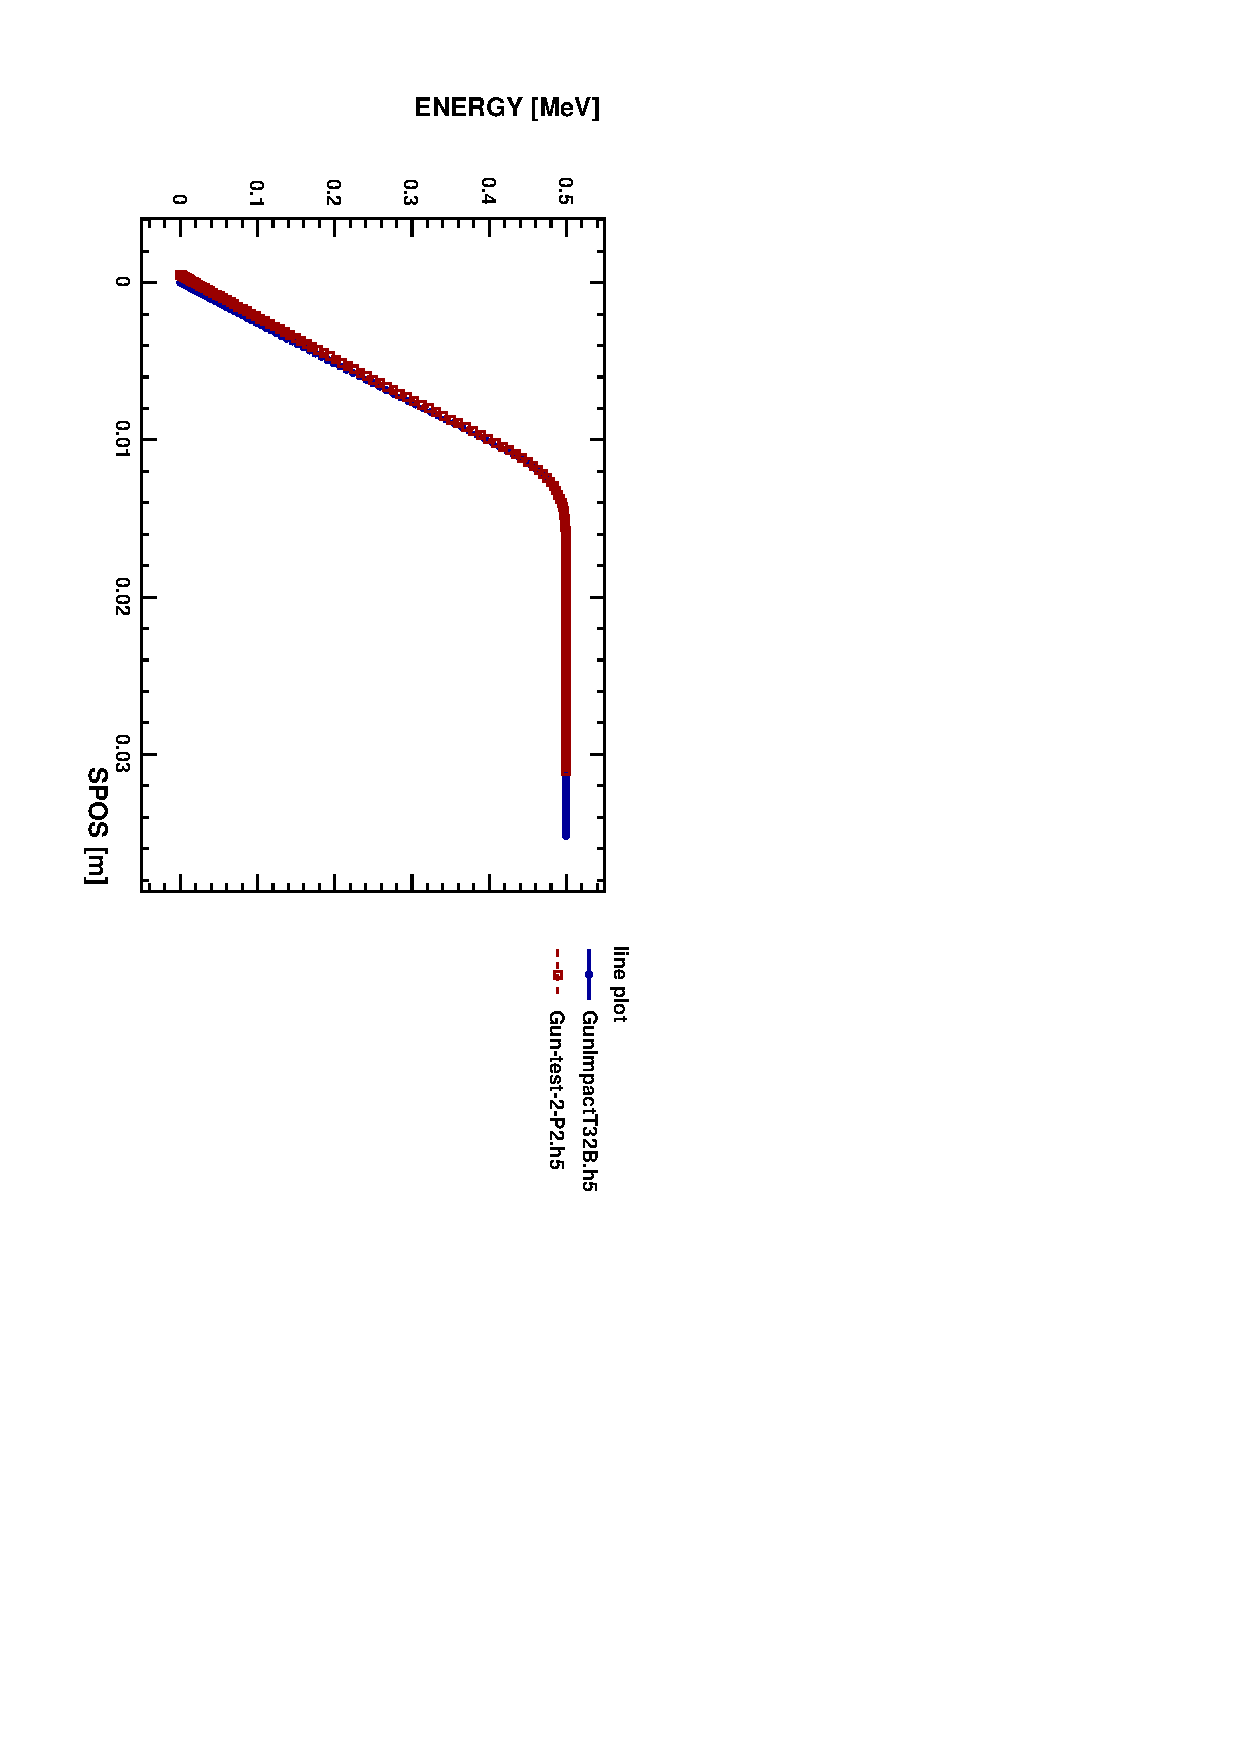
\includegraphics[width=0.60\linewidth,angle=90]{figures/Gun/GunCompEn}
   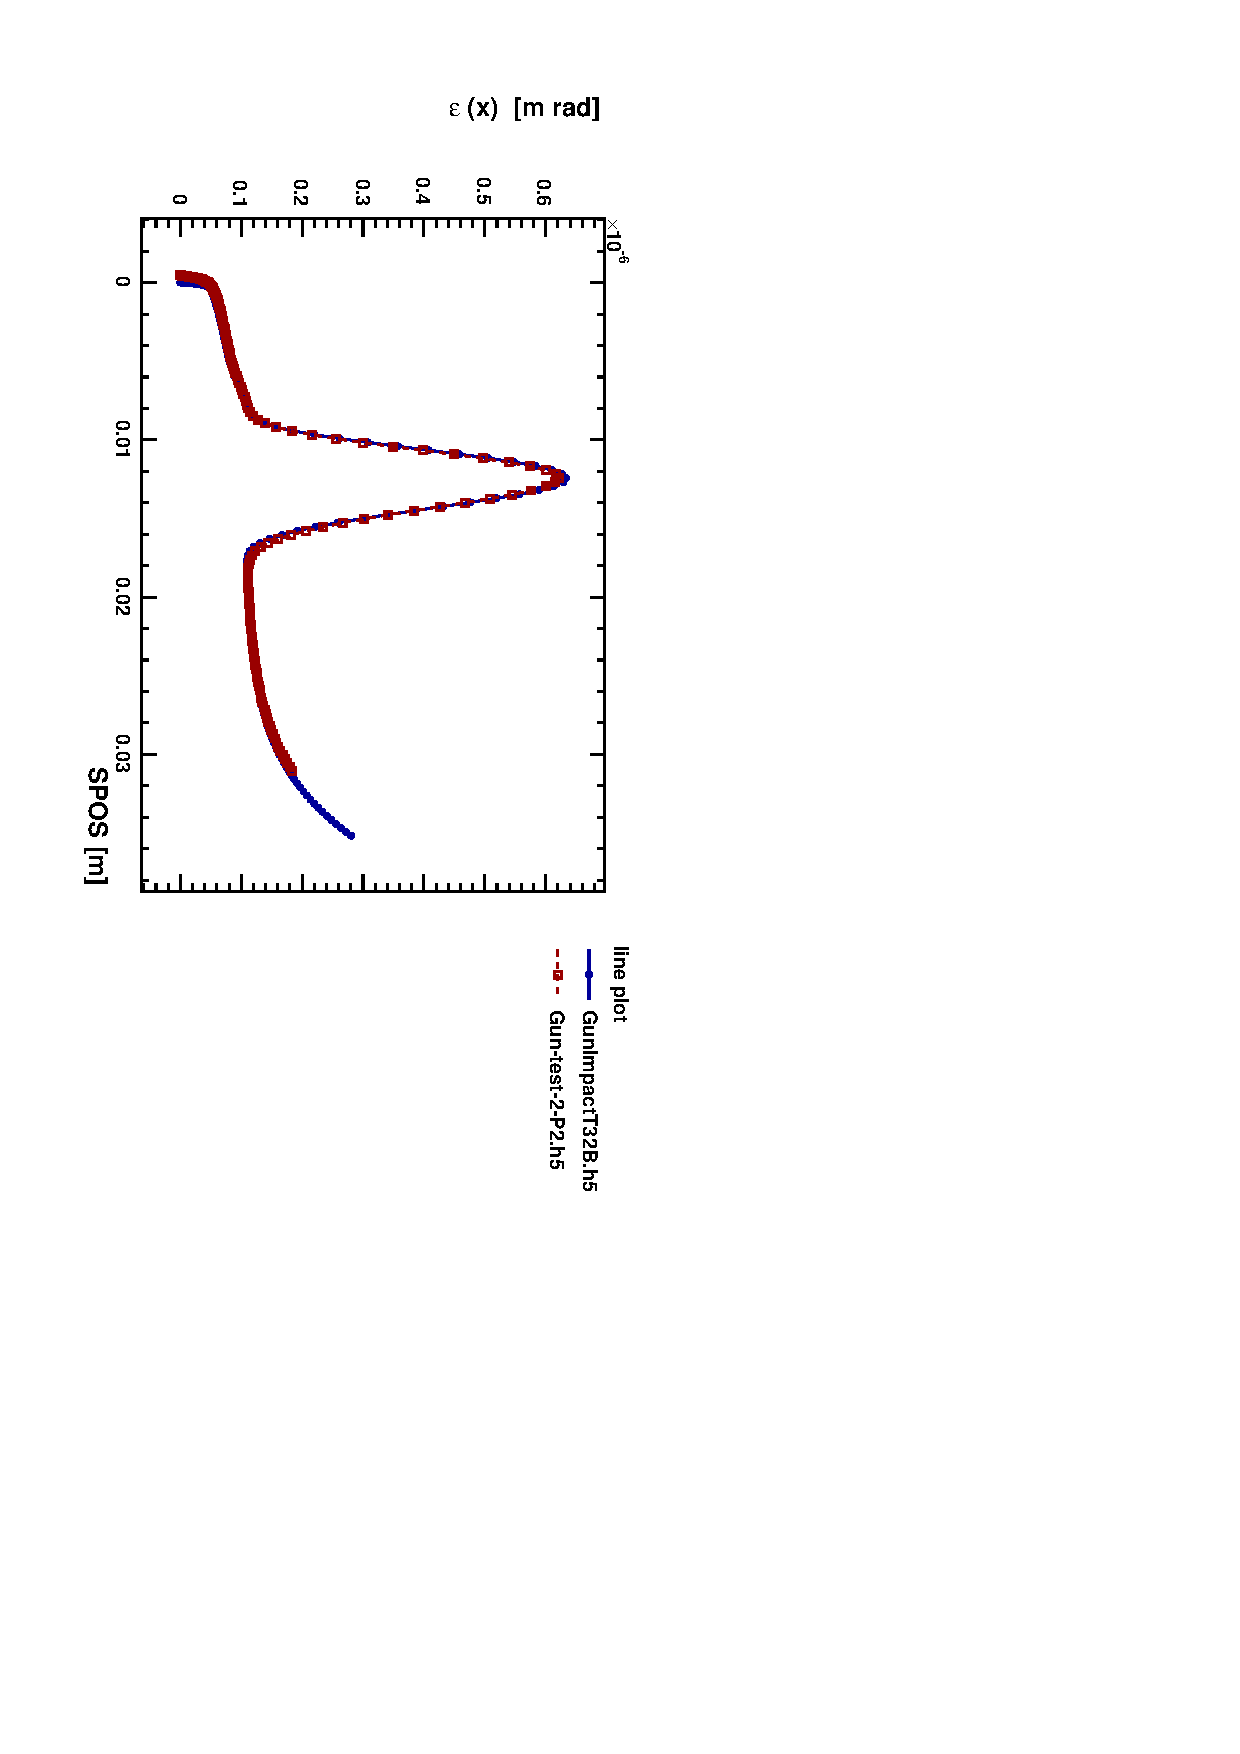
\includegraphics[width=0.60\linewidth,angle=90]{figures/Gun/GunCompEx}
   \caption{Comparison of energy and emittance in $x$ between \impactt and \opalt}   
   \label{fig:guncomp2}
 \end{center}
\end{figure}

\subsection{PSI XFEL 250 MeV Injector}
\label{sec:felinj}
\index{XFEL}
\index{INJECTOR}
\clearpage

\subsection{PSI XFEL 30 MeV Diagnostic Section}
\label{sec:feldiagsec1}
\index{XFEL}
\index{DIAGNOSTIC-1}
\begin{verbatim}
Option, ECHO=FALSE;
Option, TFS=FALSE;
Option, PSDUMPFREQ=10;

Title,string="OPAL Diagnostics test";

Edes=0.0307; //GeV
gamma=(Edes+EMASS)/EMASS;
beta=sqrt(1-(1/gamma^2));
gambet=gamma*beta;
P0 = gamma*beta*EMASS;
brho = (EMASS*1.0e9*gambet) / CLIGHT;
value,{gamma,brho,Edes,beta,gambet};

FINLB02_MSLAC40: Solenoid, L=0.001, KS=0.05, 
                                       FMAPFN="FINLB02-MSLAC.T7", ELEMEDGE=4.554;

FIND1_MQ10: Quadrupole, L=0.1, K1=2.788, ELEMEDGE=5.874;
FIND1_MQ20: Quadrupole, L=0.1, K1=-3.517, ELEMEDGE=6.074;


SCREEN: Monitor, L=0.01, ELEMEDGE=7.3867, OUTFN="Screen.h5";

FIND1:   Line = (FINLB02_MSLAC40, FIND1_MQ10, FIND1_MQ20, SCREEN);

Dist1:DISTRIBUTION, DISTRIBUTION=gauss,
                    sigmax=  1.0e-03, sigmapx=1.0e-4, corrx=0.5,
                    sigmay=  2.0e-03, sigmapy=1.0e-4, corry=-0.5,
                    sigmat=  3.0e-03, sigmapt=1.0e-4, corrt=0.0;

Fs2:FIELDSOLVER, FSTYPE=FFT, MX=32, MY=32, MT=64, 
                 PARFFTX=false, PARFFTY=false, PARFFTT=true,
                 BCFFTX=open, BCFFTY=open, BCFFTT=open,
                 BBOXINCR=1.0, GREENSF=INTEGRATED;

beam1: BEAM, PARTICLE=ELECTRON, pc=P0, NPART=1e5, 
               BFREQ=1498.953425154e6, BCURRENT=0.299598, CHARGE=-1;

Select, Line=FIND1;

track,line=FIND1, beam=beam1, MAXSTEPS=10000, DT=1.0e-12;
 run, method = "PARALLEL-T", beam=beam1, 
         fieldsolver=Fs2, distribution=Dist1;
endtrack;
Stop;
\end{verbatim}



\subsection{PSI  Injector II Cyclotron}
\label{sec:inj2}
\index{INJECTOR II}
\index{CYCLOTRON}
%%%%%%%%%%
Injector II is a separated sector cyclotron specially designed for preacceleration (inject: 870keV, extract: 72MeV )
of high intensity proton beam for Ring cyclotron. It has 4 sector magnets, two double-gap acceleration cavities 
(represented by 2 single-gap cavities here) and two single-gap flat-top cavities.  

Following is an input file of {\bfseries Single Particle Tracking mode} for PSI Injector II cyclotron.
{ \footnotesize 
\begin{verbatim}

// file name ''testinj2-1.in''

Option, TFS=FALSE;
Option, ECHO=FALSE;
Option, PSDUMPFREQ=100000;
Option, SPTDUMPFREQ=5;

Title,string="OPAL-CyclT test";

// define some physical parameters 
Edes=0.002;
gamma=(Edes+PMASS)/PMASS;
beta=sqrt(1-(1/gamma^2));
gambet=gamma*beta;
P0 = gamma*beta*PMASS;
brho = (PMASS*1.0e9*gambet) / CLIGHT;
value,{gamma,brho,Edes,beta,gambet};
phi01= 48.4812-15.0;
phi02=phi01+200.0;
phi03=phi01+1800.0;
phi04=phi01+2000.0;
phi05=(phi01+820.0)*3.0;
phi06=(phi01+2620.0)*3.0;

// define elements and beamline
inj2: Cyclotron, TYPE="Injector2", CYHARMON=10, PHIINIT=30.0, PRINIT=-0.0067,
      RINIT=392.5, SYMMETRY=1.0, RFFREQ=frequency, FMAPFN="../ZYKL9Z.NAR";

rf0: RFCavity, VOLT=0.25796, FMAPFN="../av1.dat", TYPE="SINGLEGAP", 
       FREQ=frequency, RMIN = 350.0, RMAX = 3350.0, ANGLE=35.0,
       PDIS = 0.0, GAPWIDTH = 0.0, PHI0=phi01; 

rf1: RFCavity, VOLT=0.25796, FMAPFN="../av1.dat", TYPE="SINGLEGAP", 
       FREQ=frequency, RMIN = 350.0, RMAX = 3350.0, ANGLE=55.0,
       PDIS = 0.0, GAPWIDTH = 0.0, PHI0=phi02; 

rf2: RFCavity, VOLT=0.25796, FMAPFN="../av1.dat", TYPE="SINGLEGAP", 
       FREQ=frequency, RMIN = 350.0, RMAX = 3350.0, ANGLE=215.0,  
       PDIS = 0.0, GAPWIDTH = 0.0, PHI0=phi03; 

rf3: RFCavity, VOLT=0.25796, FMAPFN="../av1.dat", TYPE="SINGLEGAP", 
       FREQ=frequency, RMIN = 350.0, RMAX = 3350.0, ANGLE=235.0,  
       PDIS = 0.0, GAPWIDTH = 0.0, PHI0=phi04; 

rf4: RFCavity, VOLT=0.06380, FMAPFN="../av3.dat", TYPE="SINGLEGAP", 
       FREQ=frequency3, RMIN = 830.0, RMAX = 3330.0, ANGLE=135.0,
       PDIS = 0.0, GAPWIDTH = 0.0, PHI0=phi05; 

rf5: RFCavity, VOLT=0.06380, FMAPFN="../av3.dat", TYPE="SINGLEGAP", 
       FREQ=frequency3, RMIN = 830.0, RMAX = 3330.0, ANGLE=315.0, 
       PDIS = 0.0, GAPWIDTH = 0.0, PHI0=phi06; 

l1:   Line = (inj2,rf0,rf1,rf2,rf3,rf4,rf5);


// define particles distribution, read from file
Dist1:DISTRIBUTION, DISTRIBUTION=fromfile,FNAME="PartDatabase.dat"; 

// define fieldsolver, useless for single particle track mode 
Fs1:FIELDSOLVER, FSTYPE=FFT, MX=64, MY=64, MT=64, 
		 PARFFTX=true, PARFFTY=true, PARFFTT=false,
		 BCFFTX=open, BCFFTY=open, BCFFTT=open;
		 
// define beam parameters
beam1: BEAM, PARTICLE=PROTON, pc=P0, SPACECHARGE=false, 
	      NPART=1, BCURRENT=0.0;

// select beamline
Select, Line=l1;

// start tracking
track,line=l1, beam=beam1, MAXSTEPS=106*2000,  STEPSPERTURN=2000;
 run, file = "track_output", turns = 1, method = "CYCLOTRON-T",
      beam=beam1, fieldsolver=Fs1, distribution=Dist1;
endtrack;
Stop;

\end{verbatim}
}
To run opal on a single node, just use this command:
{ \footnotesize 
\begin{verbatim}
 opal testinj2-1.in --commlib mpi --info 0 | tee testinj2-1.out
\end{verbatim}
}
Here shows some pictures using the resulting data from single particle tracking using \opalcycl.

Left plot of Figure \ref{fig:Inj2 reference orbit and tune} shows the accelerating orbit of reference particle. After 106 turns, the energy increases from 870KeV at
the injection point to 72.16MeV at the deflection point . 
\begin{figure}[ht]
 \begin{center} 
   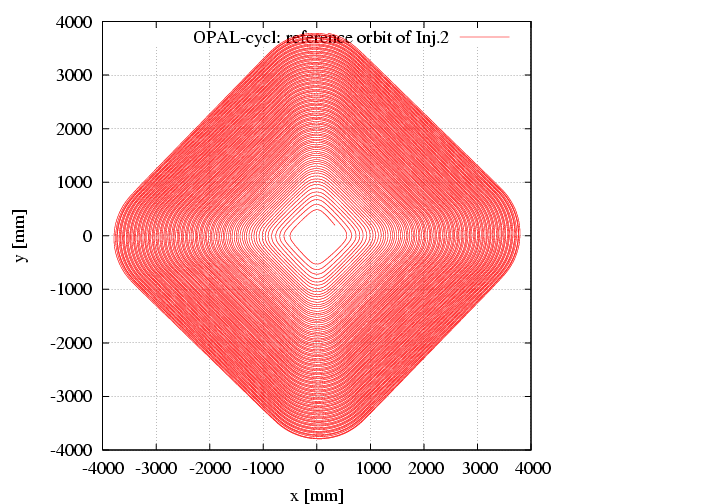
\includegraphics[width=6cm,trim=2.5cm 1.0cm 2.5cm 2.5cm]{figures/cyclotron/AEO_Injector2.png}
    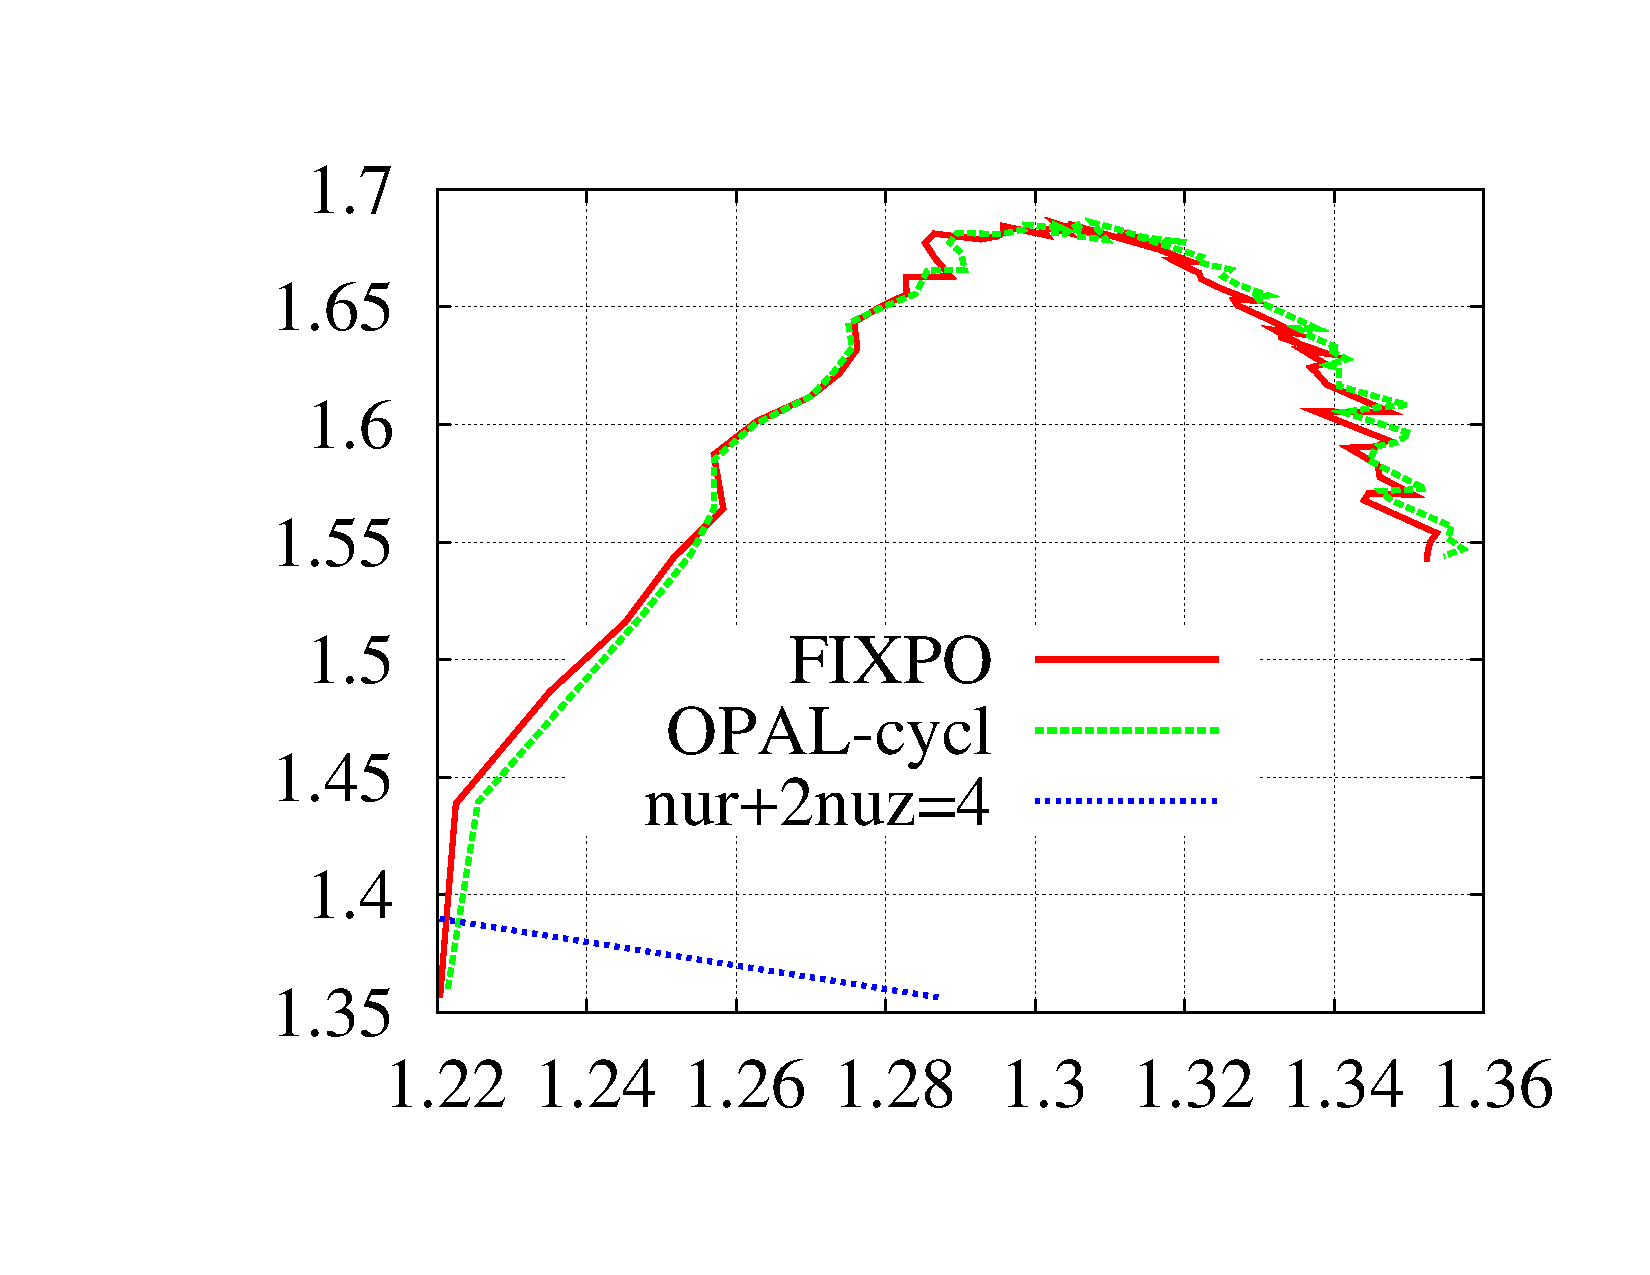
\includegraphics[width=6cm,trim=2.5cm 2.5cm 2.5cm 2.5cm]{figures/cyclotron/nurnuz_Inj2}
    \caption{Reference orbit(left) and tune diagram(right) in Injector II  }
    \label{fig:Inj2 reference orbit and tune}
 \end{center}
\end{figure}

From theoretic view, there should be an eigen ellipse for any given energy in stable area of a fixed accelerator structure. Only when the initial phase space
shape matches its eigen ellipse, the oscillation of beam envelop amplitude will get minimal and the transmission efficiency get maximal.
We can calculate the eigen ellipse by single particle tracking using betatron oscillation property of off-centered particle as following: track 
an off-centered particle and record its coordinates and momenta at the same azimuthal position for each revolution.    
Figure \ref{fig:eigen} shows the eigen ellipse at symmetric line of sector magnet for energy of 2 MeV in Injector II.
\begin{figure}[ht]
 \begin{center} 
   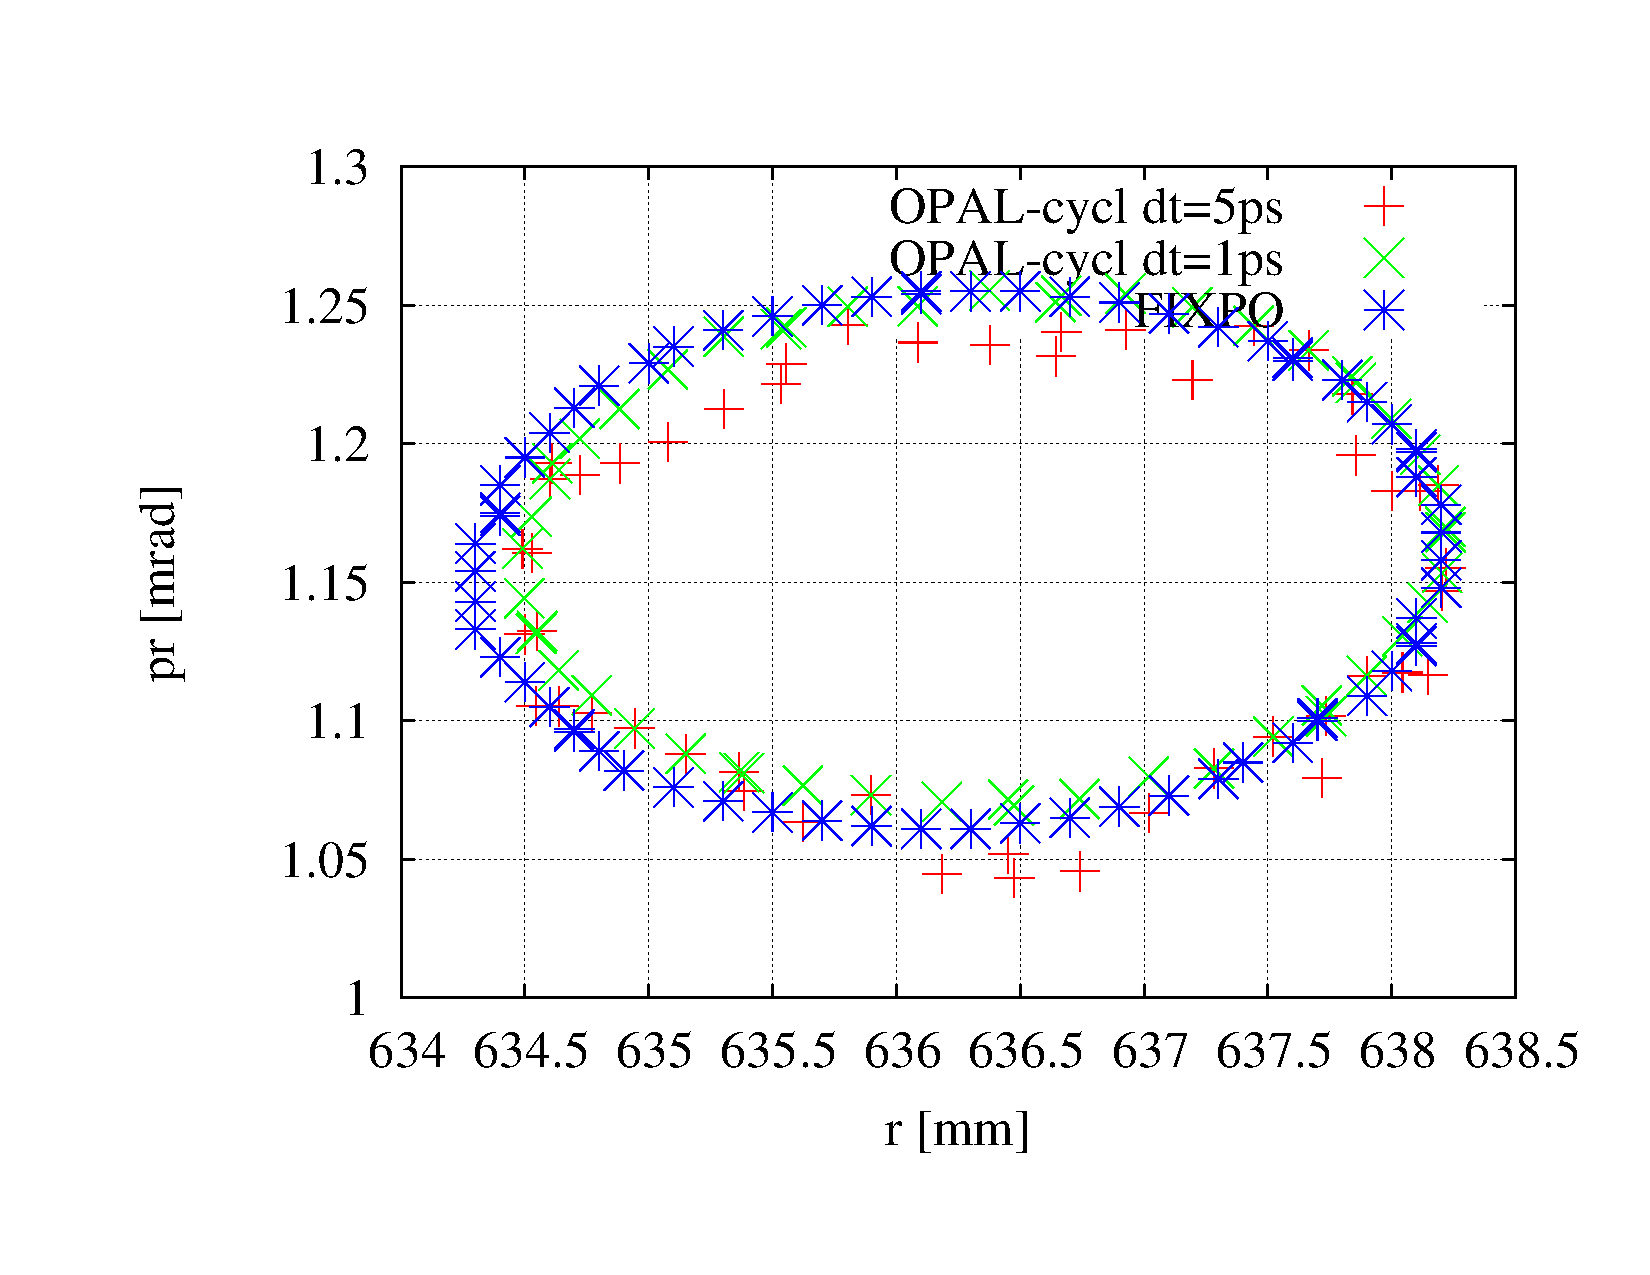
\includegraphics[width=0.45\linewidth,angle=0]{figures/cyclotron/RadialEigen_Inj2}
   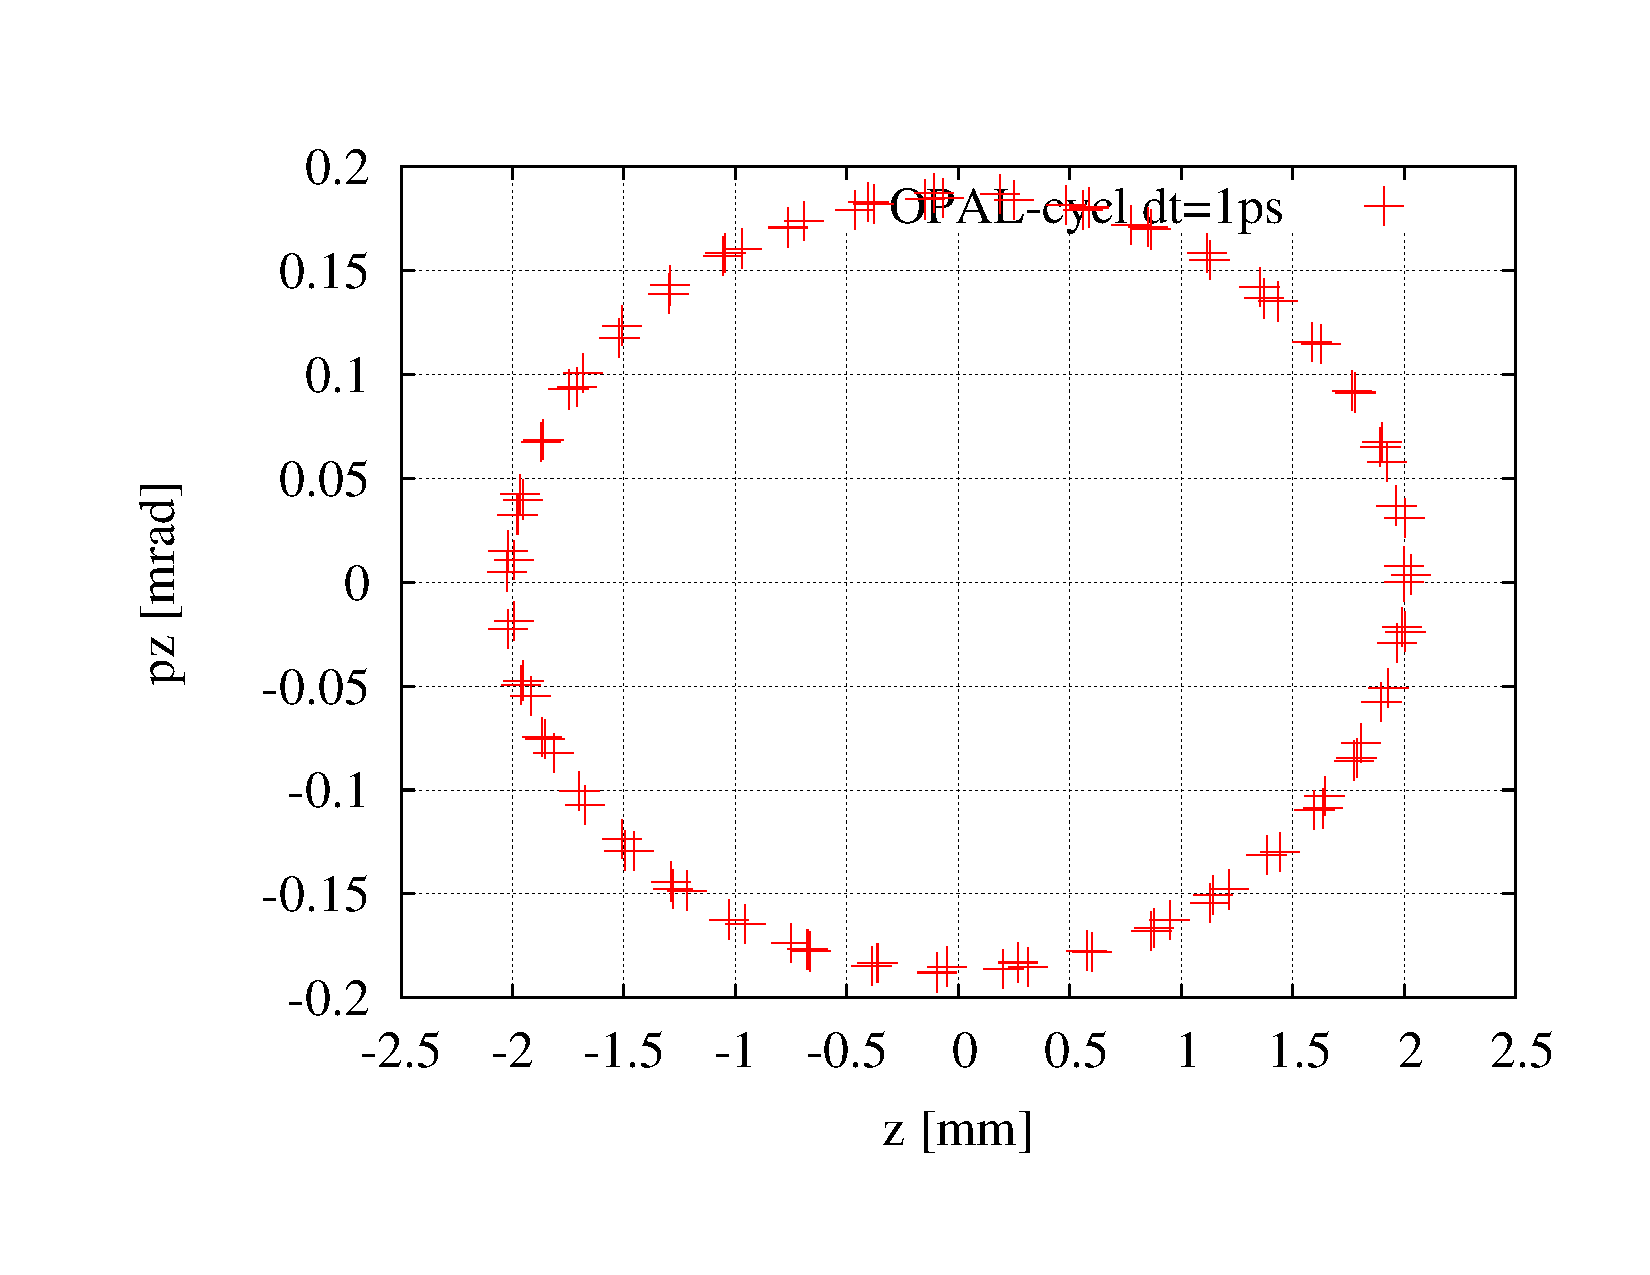
\includegraphics[width=0.45\linewidth,angle=0]{figures/cyclotron/VertEigen_Inj2}
   \caption{radial and vertical eigenellipse at 2MeV of Injector II}   
   \label{fig:eigen}
 \end{center}
\end{figure}
 
Right plot of Figure \ref{fig:Inj2 reference orbit and tune} shows very good agreement of the tune diagram by \opalcycl and FIXPO.
The trivial discrepancy should come from the methods they used.
In FIXPO, the tune values are obtained according to the crossing points of the initially displaced particle. Meanwhile, in \opalcycl, the Fourier 
analysis method is used to manipulate orbit difference between the reference particle and an initially displaced particle.
The frequency point with the biggest amplitude is the betatron tune value at the given energy.

%%%%%%%%%%%%%%
Following is the input file for single bunch tracking with space charge effects in Injector II.
%%%%%%%%%%%%%% 
{ \footnotesize
\begin{verbatim}
 
// file name ''testinj2-2.in''
// Define Option parameters 
Option, ECHO=FALSE;
Option, PSDUMPFREQ=10;
Option, SPTDUMPFREQ=5;
Option, REPARTFREQ=10;

// Define title
Title,string="OPAL-CyclT-SC test";

// define some physical parameters 
Edes=0.000870;
gamma=(Edes+PMASS)/PMASS;
beta=sqrt(1-(1/gamma^2));
gambet=gamma*beta;
P0 = gamma*beta*PMASS;
brho = (PMASS*1.0e9*gambet) / CLIGHT;

phi01= 48.4812-15.0;
phi02=phi01+200.0;
phi03=phi01+1800.0;
phi04=phi01+2000.0;
phi05=(phi01+820.0)*3.0;
phi06=(phi01+2620.0)*3.0;

frequency=50.6370;
frequency3=3.0*frequency;

// define elements and beamline
inj2: Cyclotron, TYPE="Injector2", CYHARMON=10, PHIINIT=30.0,PRINIT=-0.0067,
RINIT=392.5, SYMMETRY=1.0, RFFREQ=50.6370,FMAPFN="../../ZYKL9Z.NAR";

rf0: RFCavity, VOLT=0.25796, FMAPFN="../../Cav1.dat", TYPE="SINGLEGAP",
FREQ=50.637, RMIN = 350.0, RMAX = 3350.0, ANGLE=35.0,   PDIS = 0.0,
GAPWIDTH = 0.0, PHI0=phi01;
rf1: RFCavity, VOLT=0.25796, FMAPFN="../../Cav1.dat", TYPE="SINGLEGAP",
FREQ=50.637, RMIN = 350.0, RMAX = 3350.0, ANGLE=55.0,   PDIS = 0.0,
GAPWIDTH = 0.0, PHI0=phi02;
rf2: RFCavity, VOLT=0.25796, FMAPFN="../../Cav1.dat", TYPE="SINGLEGAP",
FREQ=50.637, RMIN = 350.0, RMAX = 3350.0, ANGLE=215.0,  PDIS = 0.0,
GAPWIDTH = 0.0, PHI0=phi03;
rf3: RFCavity, VOLT=0.25796, FMAPFN="../../Cav1.dat", TYPE="SINGLEGAP",
FREQ=50.637, RMIN = 350.0, RMAX = 3350.0, ANGLE=235.0,  PDIS = 0.0,
GAPWIDTH = 0.0, PHI0=phi04;
rf4: RFCavity, VOLT=0.06380, FMAPFN="../../Cav3.dat", TYPE="SINGLEGAP",
FREQ=151.911, RMIN = 830.0, RMAX = 3330.0, ANGLE=135.0, PDIS = 0.0,
GAPWIDTH = 0.0, PHI0=phi05;
rf5: RFCavity, VOLT=0.06380, FMAPFN="../../Cav3.dat", TYPE="SINGLEGAP",
FREQ=151.911, RMIN = 830.0, RMAX = 3330.0, ANGLE=315.0, PDIS = 0.0,
GAPWIDTH = 0.0, PHI0=phi06;

l1:   Line = (inj2,rf0,rf1,rf2,rf3,rf4,rf5);

// define particles distribution, generate Gaussion type
Dist1:DISTRIBUTION, DISTRIBUTION=gauss,
sigmax=  2.0e-03, sigmapx=1.0e-7, corrx=0.0,
sigmay=  2.0e-03, sigmapy=1.0e-7, corry=0.0,
sigmat=  2.0e-03, sigmapt=1.8e-4, corrt=0.0;

// define parallel FFT fieldsolver, parallel in x y direction
Fs1:FIELDSOLVER, FSTYPE=FFT, MX=32, MY=32, MT=32, 
		 PARFFTX=true, PARFFTY=true, PARFFTT=false,
		 BCFFTX=open, BCFFTY=open, BCFFTT=open,BBOXINCR=5;

// define beam parameters
beam1: BEAM, PARTICLE=PROTON, pc=P0, SPACECHARGE=true,
       NPART=1e5, BCURRENT=3.0E-3, CHARGE=1.0, BFREQ= frequency;

// select beamline
Select, Line=l1;

// start tracking
track,line=l1, beam=beam1, MAXSTEPS=106*2000,  STEPSPERTURN=2000;
 run, file = "track_output", turns = 1, method = "CYCLOTRON-T", 
      beam=beam1, fieldsolver=Fs1, distribution=Dist1;
endtrack;
Stop;
\end{verbatim}
}
To run opal on single node, just use this command:
{ \footnotesize 
\begin{verbatim}
 # opal testinj2-2.in --commlib mpi --info 0 | tee testinj2-2.out
\end{verbatim}
}
To run opal on N nodes in parallel environment interactively, use this command instead:
{ \footnotesize 
\begin{verbatim}
 # mpirun -np N opal testinj2-2.in  --commlib mpi 
   --info 0 | tee testinj2-2.out
\end{verbatim}
 }
If restart a job from the last step NSTEP of an existing $.h5$ file, add a new argument like this: 
{ \footnotesize 
\begin{verbatim}
 # mpirun -np N opal testinj2-2.in --restart NSTEP 
   --commlib mpi --info 0 | tee testinj2-2.out
\end{verbatim}
}
Figure \ref{fig:cyclParameters} and \ref{fig:cyclphasespace} are from preliminary simulation results.
They are generated by H5partROOT code.   
\begin{figure}[ht]
  \begin{center} 
    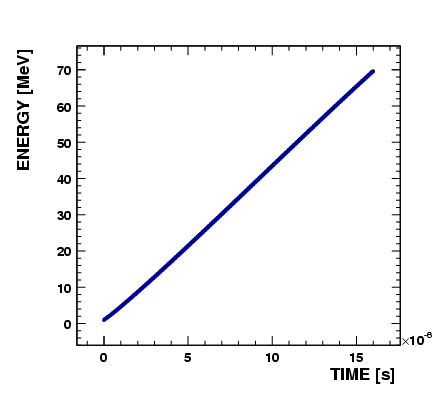
\includegraphics[width=0.45\linewidth]{figures/cyclotron/Inj2-ENERGY-TIME.png}
    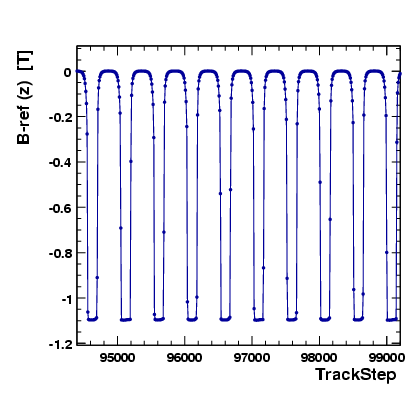
\includegraphics[width=0.45\linewidth]{figures/cyclotron/Inj2-B-ref-z-TrackStep.png}
    \caption{Energy Vs. time (left) and external B field Vs. trackstep (Right, only show for about 2 turns)}
    \label{fig:cyclParameters}
  \end{center}
\end{figure}

\begin{figure}[ht]
  \begin{center} 

    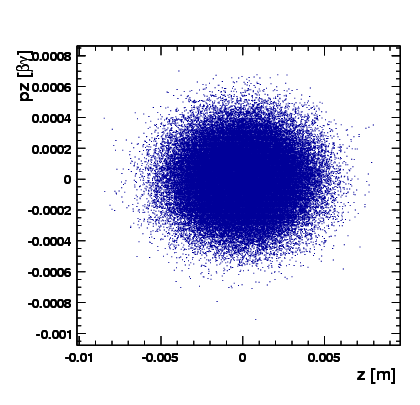
\includegraphics[width=0.3\linewidth]{figures/cyclotron/Inj2-z-pz-step-870KeV.png}
    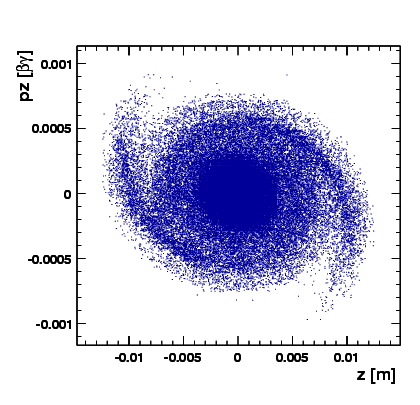
\includegraphics[width=0.3\linewidth]{figures/cyclotron/Inj2-z-pz-step-15MeV.png}
    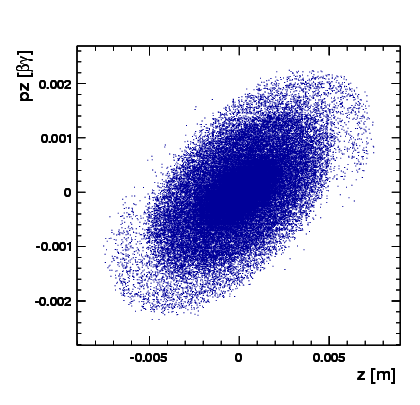
\includegraphics[width=0.3\linewidth]{figures/cyclotron/Inj2-z-pz-step-30MeV.png}
    \caption{Vertical phase at different energy from left to right: 0.87,15 and 35( MeV}
    \label{fig:cyclphasespace}
  \end{center}
\end{figure}

%%%%%%%%%%%%%%
\subsection{PSI  Ring Cyclotron}
\label{sec:Ring}
\index{RING}
\index{CYCLOTRON}
From the view of numerical simulation, the difference between Injector II and Ring cyclotron comes from two aspects:
\begin{description}
\item[B Field] The structure of Ring is totally symmetric, the field on median plain is periodic 
along azimuthal direction, \opalcycl take this advantage to only store 1/8 field data to save memory.

\item[RF Cavity] In the Ring, all the cavities are typically single gap with some parallel displacement from its
radial position.\opalcycl have an argument \texttt{PDIS} to manipulate this issue.  
\end{description}
\begin{figure}[ht]
  \begin{center} 
    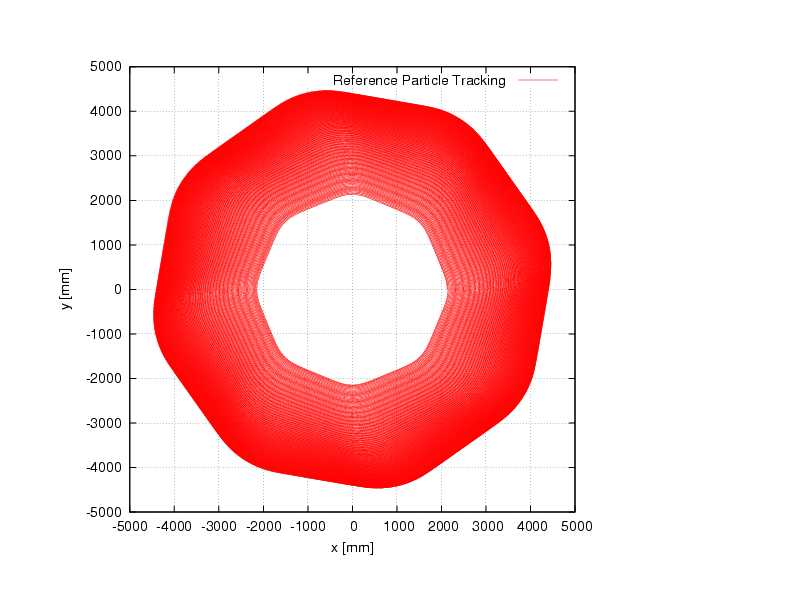
\includegraphics[width=6cm,trim=2.5cm 2.5cm 2.5cm 2.5cm]{figures/cyclotron/AEO_Ring.png}
    \includegraphics[width=6cm,trim=2.5cm 2.5cm 2.5cm 2.5cm]{figures/cyclotron/nurnuz_Ring}
    \caption{Reference orbit(left) and tune diagram(right) in Ring cyclotron }
    \label{fig:Ring reference orbit and tune}
  \end{center}
\end{figure}
Figure \ref{fig:Ring reference orbit and tune} shows single particle tracking result and tune calculation result in PIS Ring cyclotron.
Limited by size of the user guide, we don't plan to show too much details as in Injector II.

\clearpage
\subsection{CERN SPS Lattice}
\label{sec:sps}
\index{SPS}
The CERN SPS lattice may be represented using the following beam elements:
\begin{verbatim}
QF:QUADRUPOLE,...; // focusing quadrupole
QD:QUADRUPOLE,...; // defocusing quadrupole
B1:RBEND,...;      // bending magnet of type 1
B2:RBEND,...;      // bending magnet of type 2
DS:DRIFT,...;      // short drift space
DM:DRIFT,...;      // drift space replacing two bends
DL:DRIFT,...;      // long drift space
\end{verbatim}
The SPS machine is represented by the lines
\begin{verbatim}
SPS:   LINE=(6*SUPER);
SUPER: LINE=(7*P44,INSERT,7*P44);
INSERT:LINE=(P24,2*P00,P42);
P00:   LINE=(QF,DL,QD,DL);
P24:   LINE=(QF,DM,2*B2,DS,PD);
P42:   LINE=(PF,QD,2*B2,DM,DS);
P44:   LINE=(PF,PD);
PD:    LINE=(QD,2*B2,2*B1,DS);
PF:    LINE=(QF,2*B1,2*B2,DS);
\end{verbatim}
In order not to overload the example,
small gaps between magnetic elements have been omitted.

\subsection{LEP Lattice}
\label{sec:lep}
\index{LEP}
A preliminary description of LEP has been given in the
\bibref{LEP pink book}{LEP}.
Translation of those element sequences to the \opal input format gives:
\begin{verbatim}
LEP: LINE=(4*SUP);
SUP: LINE=(OCT,-OCT);
OCT: LINE=(LOBS,RFS,DISS,ARC,DISL,RFL,LOBL);
LOBS:LINE=(L1,QS1,L2,QS2,L3,QS3,L4,QS4);
RFS: LINE=(L5,QS5,L5,QS6,L5,2*(QS7,L5,QS8,L5));
DISS:LINE=(QS11,L25,BW,L22,QS12,L25,B4,L22,QS13,L25,B4,
           L22,QS14,L25,B4,L31,QS15,L25,B4,L32,SF,L23,QS16);
ARC: LINE=(L21,B6,L22,SD,L23,QD,
           7*(CELL(SF1,SD1),CELL(SF,SD)),CELL(SF1,SD1),
           L24,B6,L41,QF,L21,B6,L22,SD4,L23,QD,
           7*(CELL(SF4,SD3),CELL(SF3,SD4)),CELL(SF4,SD3),
           L24,B6,L22,SF3,L23);
DISL:LINE=(QL16,L34,B4,L22,QL15,L33,B4,L22,QL14,L25,B4,
           L22,QL13,L25,B4,L22,QL12,L25,BW,L22,QL11);
RFL: LINE=(2*(L5,QL8,L5,QL7),L5,QL6,L5,QL5,L5);
LOBL:LINE=(QL4,L14,QL3,L13,QL2,L12,QL1,L11);
BW:  LINE=(W,L26,W);
B4:  LINE=(B,L26,B);
B6:  LINE=(B,L26,B,L26,B);
CELL(SF,SD):LINE=(L24,B6,L22,SF,L23,QF,L21,B6,L22,SD,L23,QD);
\end{verbatim}
Here the element definitions have been left out to save space.
